\documentclass{article}
\usepackage[utf8]{inputenc}
\usepackage{tabularx} % extra features for tabular environment
\usepackage{amsmath}  % improve math presentation
\usepackage{graphicx} % takes care of graphic including machinery
\usepackage{xspace}
\usepackage{tikz}
\usepackage{pdfpages}
\usepackage{enumitem}
\usetikzlibrary{babel}
\usepackage[american]{circuitikz}
\usetikzlibrary{calc}
\usepackage{float}
\usepackage{siunitx}
\usepackage{pgfplots}
\usepackage[skins,theorems]{tcolorbox}
\tcbset{highlight math style={enhanced,
  colframe=red,colback=white,arc=0pt,boxrule=1pt}}
\pgfplotsset{width=10cm,compat=1.9}
\usepackage[margin=1in,letterpaper]{geometry} % decreases margins
\usepackage{cite} % takes care of citations
\usepackage[final]{hyperref} % adds hyper links inside the generated PDF file
\hypersetup{
colorlinks=true,       % false: boxed links; true: colored links
linkcolor=blue,        % color of internal links
citecolor=blue,        % color of links to bibliography
filecolor=magenta,     % color of file links
urlcolor=blue        
}

\begin{document}

\title{{\textbf{ASSIGNMENT 7}}}
\author{\textbf{TADIPATRI UDAY KIRAN REDDY}\\\textbf{EE19BTECH11038}}
\maketitle

\section*{\hfil Problem 1}
\subsection*{(a)}
% FIG
\begin{gather*}
	I_D = 1A\\
	V_o = 1.3 + V_s
\end{gather*}
\subsection*{(b)}
\begin{gather*}
NoisePSD = 1.69*2*1.6*10^{-19}*1\\
\implies \tcbhighmath[drop fuzzy shadow]{NoisePSD = 5.41e-19 W/Hz}
\end{gather*}
\subsection*{(c)}
Here the gain is 1, any addition of resistance in series will reduce the gain. Thus there is \textbf{no resistance which can give the same gain}.
\section*{\hfil Problem 2}
For the total chain,
\begin{gather*}
	F_{eff} = 1 + \frac{V_{n, in_{3}}^2}{(A_{p1}A_{p2}A_{p3})^2V_{n, s}^2} + \frac{V_{n, in_{2}}^2}{(A_{p1}A_{p2})^2V_{n, s}^2} + \frac{V_{n, in_{1}}^2}{(A_{p1})^2V_{n, s}^2}
\end{gather*}
Take intermediate stage say ith stage,
\begin{gather*}
	F_i = \frac{A_{pi}^2V_{n, in_i}^2 + V_{n, in_{i+1}}^2}{A_{pi}^2V_{n, in_i}^2} = 1 + \frac{V_{n, in_{i+1}}^2}{A_{pi}^2V_{n, in_i}^2}
\end{gather*}
And since, $A_{pi} = \frac{V_{in_{i+1}}}{V_{in_{i}}}$.
\begin{gather*}
	\tcbhighmath[drop fuzzy shadow]{F_{eff} = 1 + (1-F_1)(1-F_2)(1-F_3) + (1-F_1)(1-F_2) + (1-F_1)}
\end{gather*}
\section*{\hfil Problem 3}
We find gain from input to output and just multiply the input noise PSD with square of magnitude of gain.
\subsection*{(a)}
\begin{gather*}
	\frac{V_o}{V_{in}} = \frac{1}{sCR + 1}\\
	Noise PSD = AvAv^*V_n^2
	\implies \tcbhighmath[drop fuzzy shadow]{NoisePSD = \frac{1}{1 + (\omega CR)^2}}
\end{gather*}
\subsection*{(b)}
\begin{gather*}
	\frac{V_o}{V_{in}} = \frac{1}{s^2LC + sCR + 1}\\
	\implies \tcbhighmath[drop fuzzy shadow]{NoisePSD = \frac{V_n^2}{(1 - {\omega}^2 LC)^2 + (\omega CR)^2}}
\end{gather*}
\subsection*{(c)}
\begin{gather*}
	\frac{V_{o1}}{V_{in}} = \frac{s^2LC_2 + 1}{s^3RLC_1C_2 + s^2LC_2 + sR(C_1 + C_2) + 1}\\
	\implies \tcbhighmath[drop fuzzy shadow]{NoisePSD_1 = V_n^2\frac{(1 - {\omega}^2LC_2)^2}{(1 - {\omega}^2LC_2)^2 + ({\omega}^3RLC_1C_2 - {\omega}R(C_1 + C_2))^2}}\\
	\frac{V_{o2}}{V_{in}} = \frac{1}{s^3RLC_1C_2 + s^2LC_2 + sR(C_1 + C_2) + 1}\\
	\implies \tcbhighmath[drop fuzzy shadow]{NoisePSD_2 = V_n^2\frac{1}{(1 - {\omega}^2LC_2)^2 + ({\omega}^3RLC_1C_2 - {\omega}R(C_1 + C_2))^2}}\\
\end{gather*}
\section*{\hfil Problem 4}

\section*{\hfil Problem 5}
We can find Z-parameters for both the models and just equate corresponding parameters.
\subsection*{Model 1}
\begin{figure}[H]
	\centering
	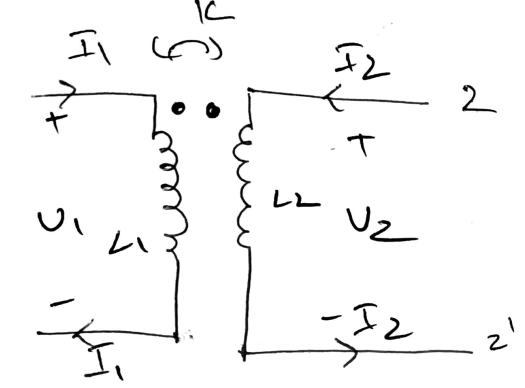
\includegraphics[scale=0.4]{./figs/5m1.png}
\end{figure}
\begin{gather*}
V_1 = sL_1I_1 + sMI_2\\
V_2 = sMI_1 + sL_2I_2\\
M = K\sqrt{L_1L_2}
\end{gather*}
\subsection*{Model 2}
\begin{figure}[H]
	\centering
%	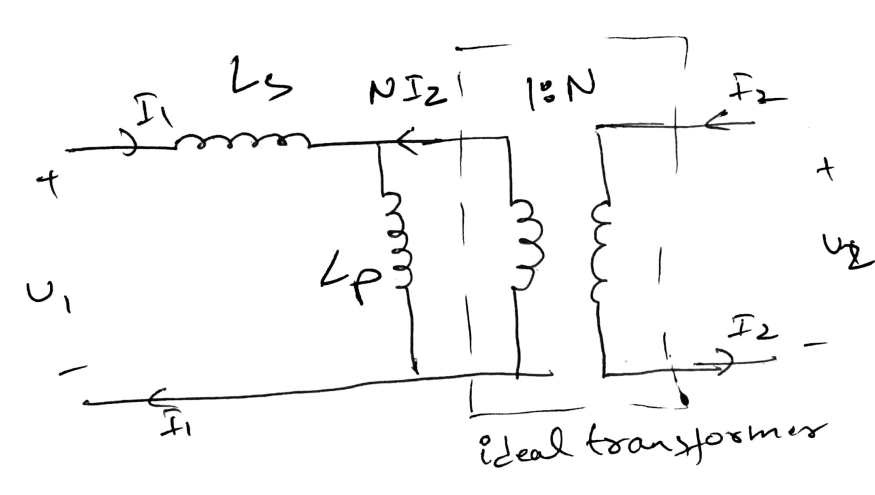
\includegraphics[scale=0.4hot]{./figs/5m2.png}
\end{figure}
\begin{gather*}
V_1 = s(L_s + L_p)I_1 + sNL_pI_2\\
V_2 = sNL_pI_1 + sN^2L_pI_2
\end{gather*}
From above equations we conclude that,
\begin{gather*}
L_1 = L_s + L_p\\
NL_p = K\sqrt{L_1L_2}\\
N^2L_p = L_2\\
\implies \tcbhighmath[drop fuzzy shadow]{N =  \frac{1}{K}\sqrt{\frac{L_2}{L_1}}}\\
\implies \tcbhighmath[drop fuzzy shadow]{L_p = K^2L_1}
\implies \tcbhighmath[drop fuzzy shadow]{L_s = (1 - K^2)L_1}
\end{gather*}
\section*{\hfil Problem 6}
At receiver,
\begin{gather*}
NF = SNR_{in} - SNR_{out} = 10dB\\
SNR_{in} = 10dB + SNR_{out} \ge 10dB\\
\implies P_{Rx} \ge P_{noise} + 10dB \implies P_{Tx} - P_{atten} \ge P_{noise} + 10dB\\
\implies P_{atten} \le  P_{Tx} - (P_{noise} + 10dB)
\end{gather*}
Assuming the circuits are matched, $P_{noise}$ would be $-173.8 + 10log_{10}B$ which is -123.8bB. Therefore,
\begin{gather*}
\tcbhighmath[drop fuzzy shadow]{P_{atten} \le 143.8dB}
\end{gather*}
Maximum of 143.8dB of atmospheric attenuation is allowed.
\end{document}